\paragraph{Monai VAE}\mbox{}\\

\paragraph{Model configuration}\mbox{}\\
\begin{table}[h!]
\centering
\begin{tabular}{|l|l|}
\hline
\textbf{Parameter} & \textbf{Value} \\
\hline
\multicolumn{2}{|c|}{\textbf{Training}} \\
\hline
Batch Size & 5 \\
\hline
Seed & 42 \\
\hline
Epochs & 1500 \\
\hline
Training Ratio & 0.9 \\
\hline
Number of Nodes & 1 \\
\hline
Device & CUDA \\
\hline
\multicolumn{2}{|c|}{\textbf{Model}} \\
\hline
Learning Rate & 0.0002 \\
\hline
Scan Shape & [1, 128, 128, 32] \\
\hline
Beta1 & 0.5 \\
\hline
Beta2 & 0.999 \\
\hline
Adversarial Weight & 0.01 \\
\hline
Perceptual Weight & 0.005 \\
\hline
KL Weight & 1e-5 \\
\hline
Fake 3D Ratio & 0.2 \\
\hline
Autoencoder Warm-Up Epochs & 5 \\
\hline
\multicolumn{2}{|c|}{\textbf{Dataset}} \\
\hline
Caching & Disk \\
\hline
Path & /ravana/d3d\_work/micorl/data/ct\_images\_prostate\_32fixed/ \\
\hline
Image Size & 128 \\
\hline
Number of Slices & 32 \\
\hline
Window Width & 400 \\
\hline
Window Level & 60 \\
\hline
\end{tabular}
\caption{Parameters for the MONAI Autoencoder}
\label{table:monai_autoencoder_params}
\end{table}


\paragraph{Training}\mbox{}\\

\begin{figure}[H]
\minipage{0.49\textwidth}
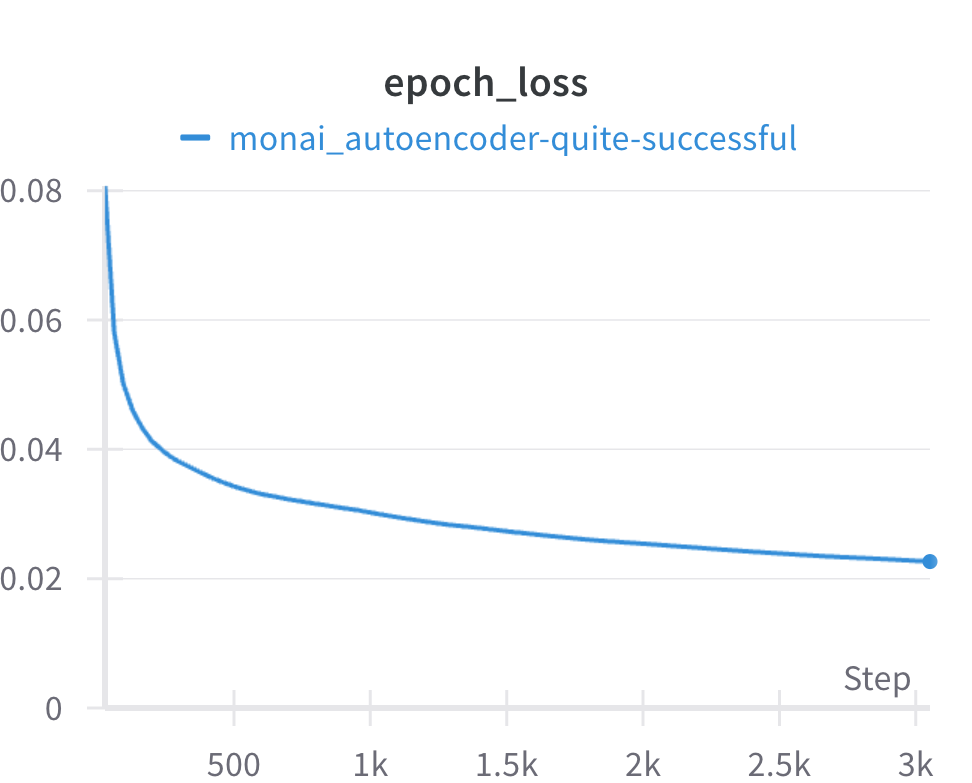
\includegraphics[width=\linewidth]{detailed_engineering/Monai Autoencoder/charts/epoch_loss.png}
\caption{}
\endminipage\hfill
\minipage{0.49\textwidth}
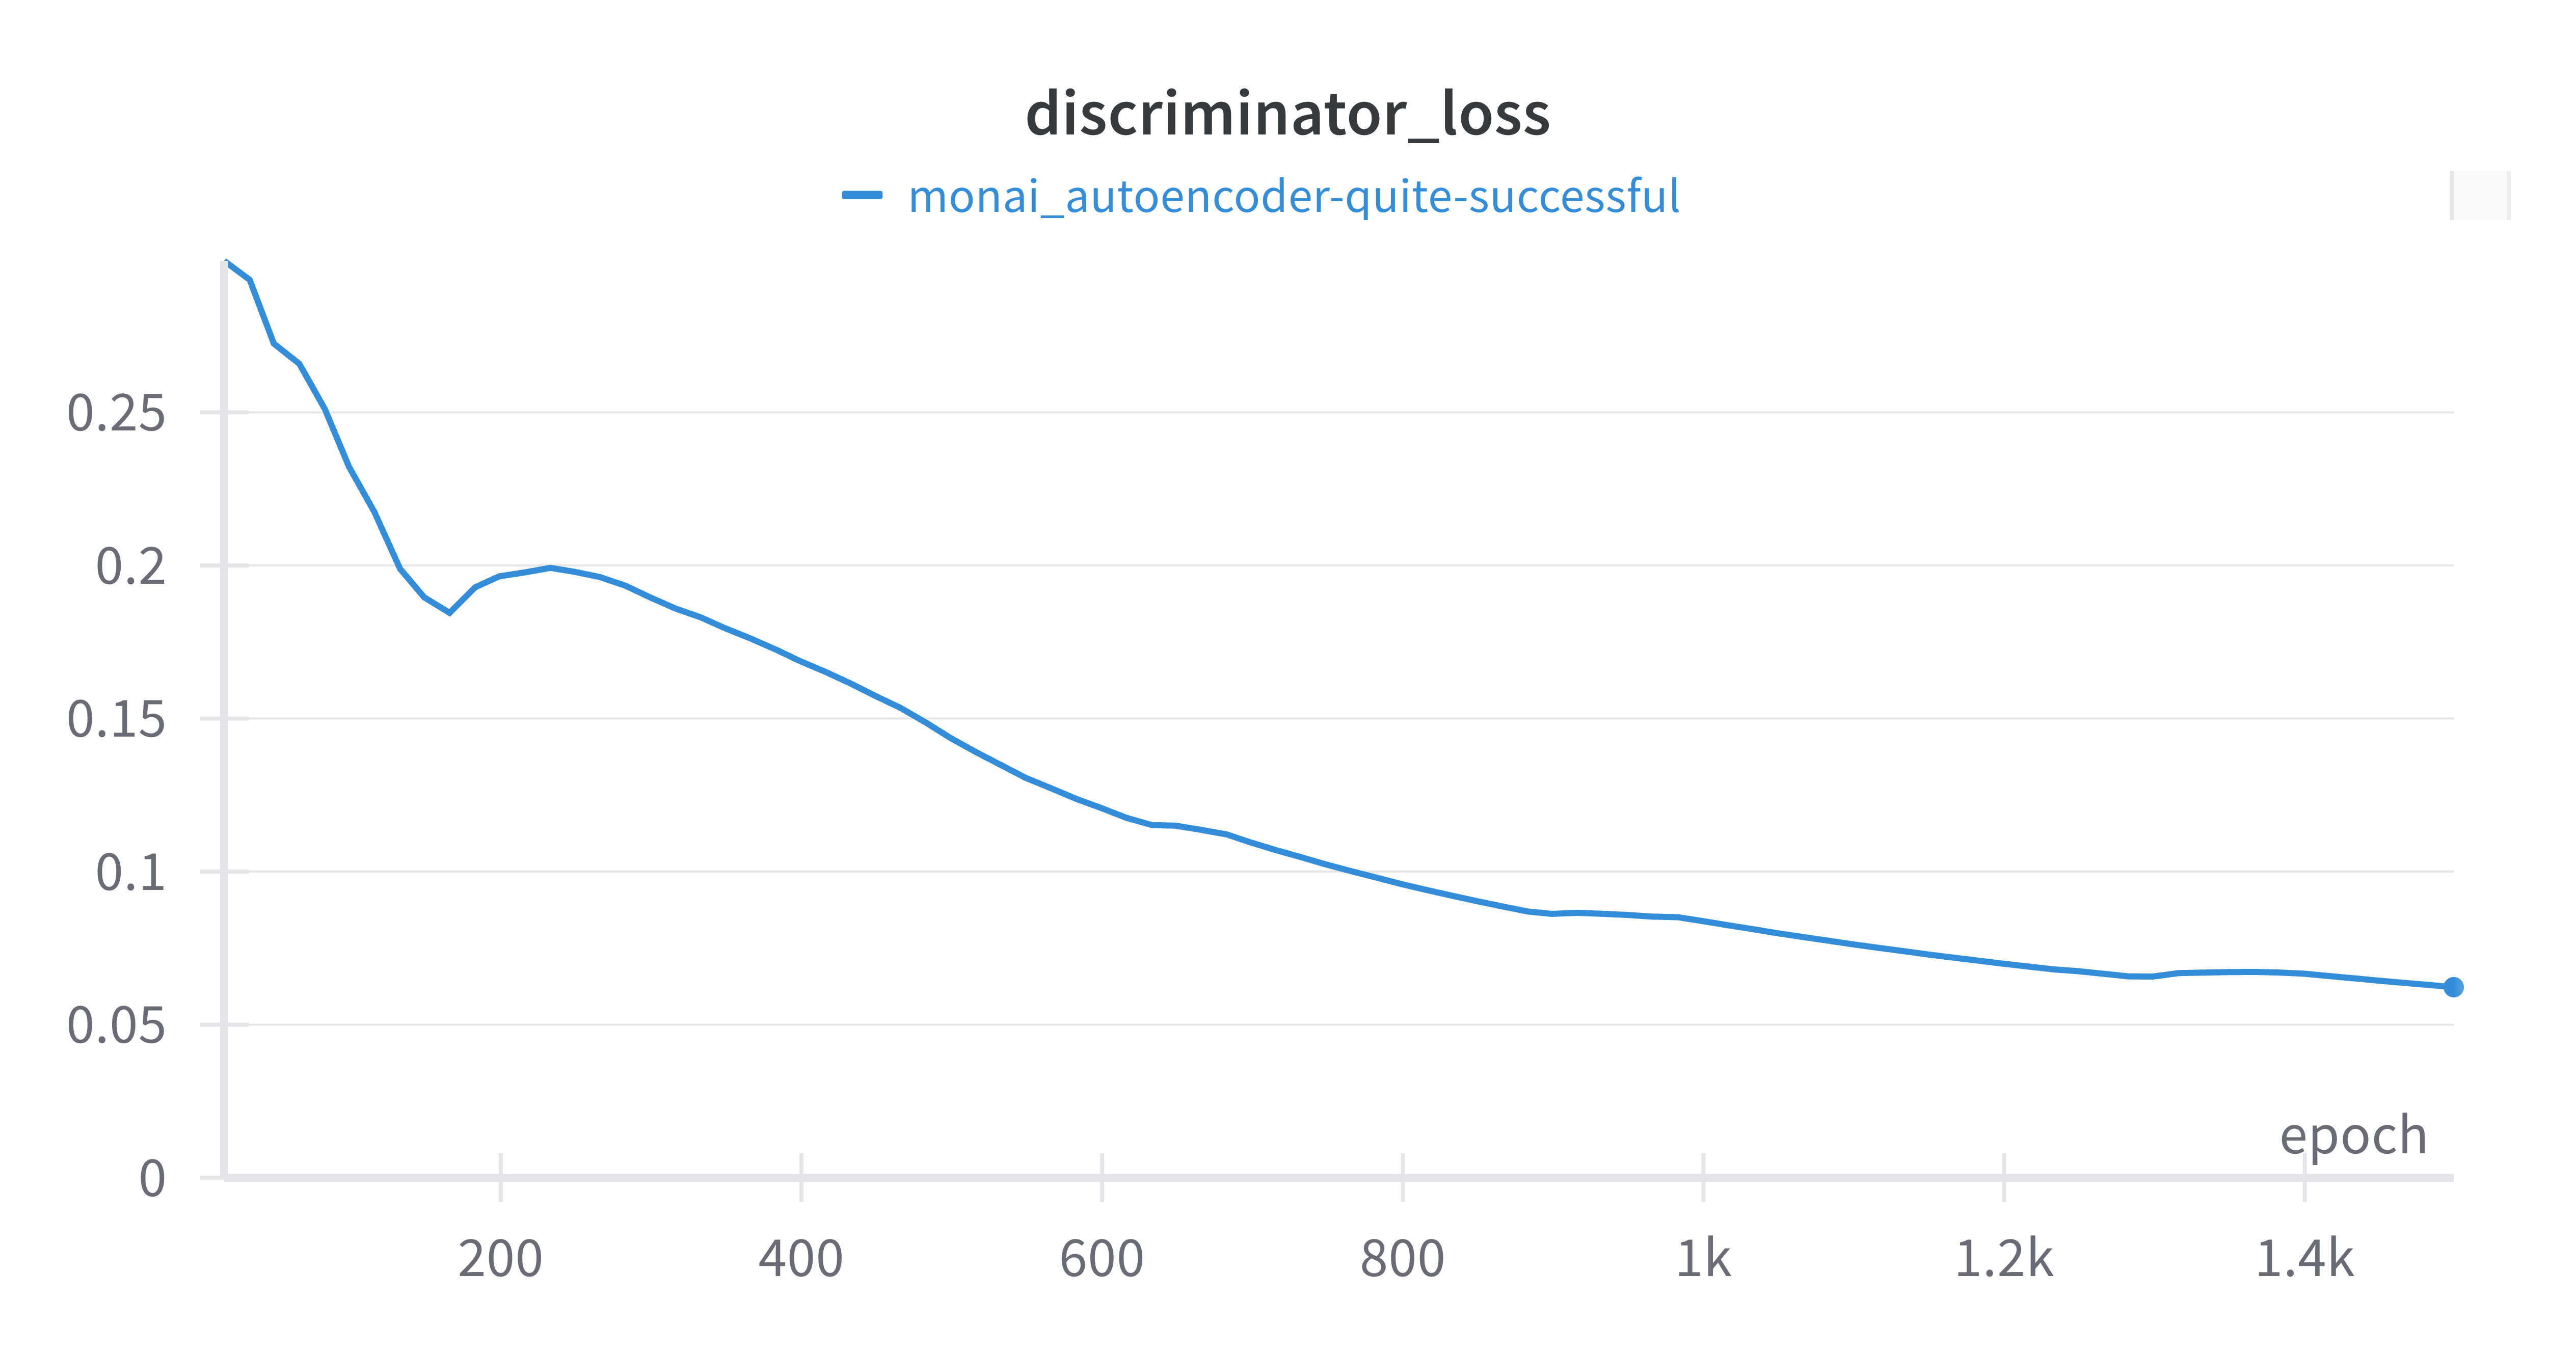
\includegraphics[width=\linewidth]{detailed_engineering/Monai Autoencoder/charts/discriminator_loss.png}
\caption{}
\endminipage
\end{figure}

\begin{figure}[H]
\minipage{0.49\textwidth}
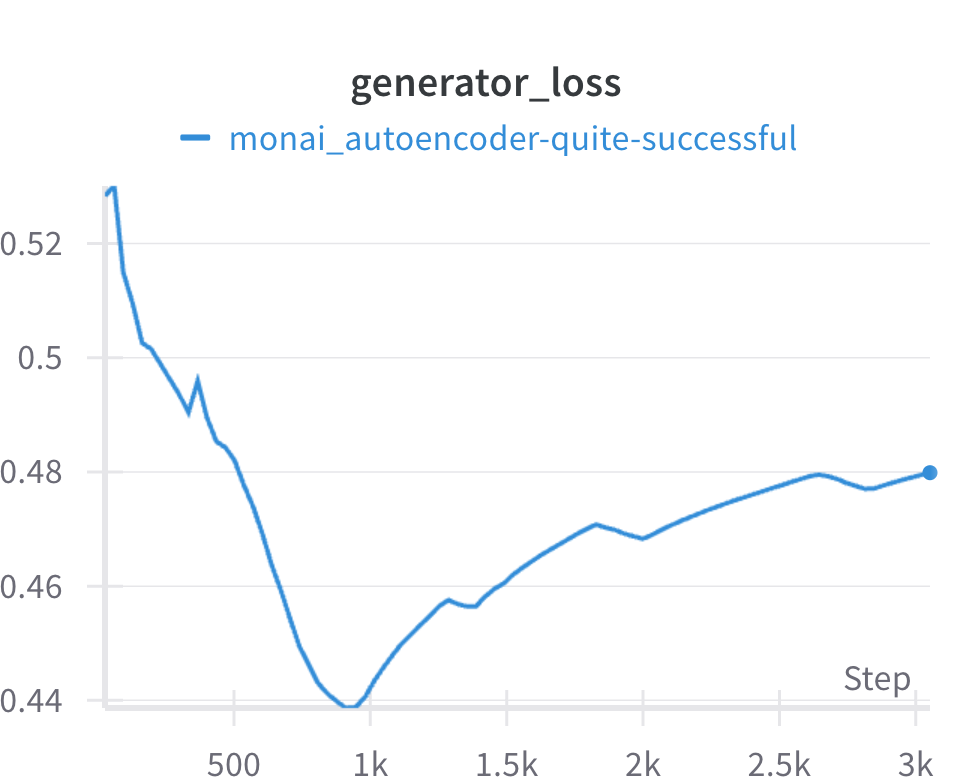
\includegraphics[width=\linewidth]{detailed_engineering/Monai Autoencoder/charts/generator_loss.png}
\caption{}
\endminipage\hfill
\minipage{0.49\textwidth}
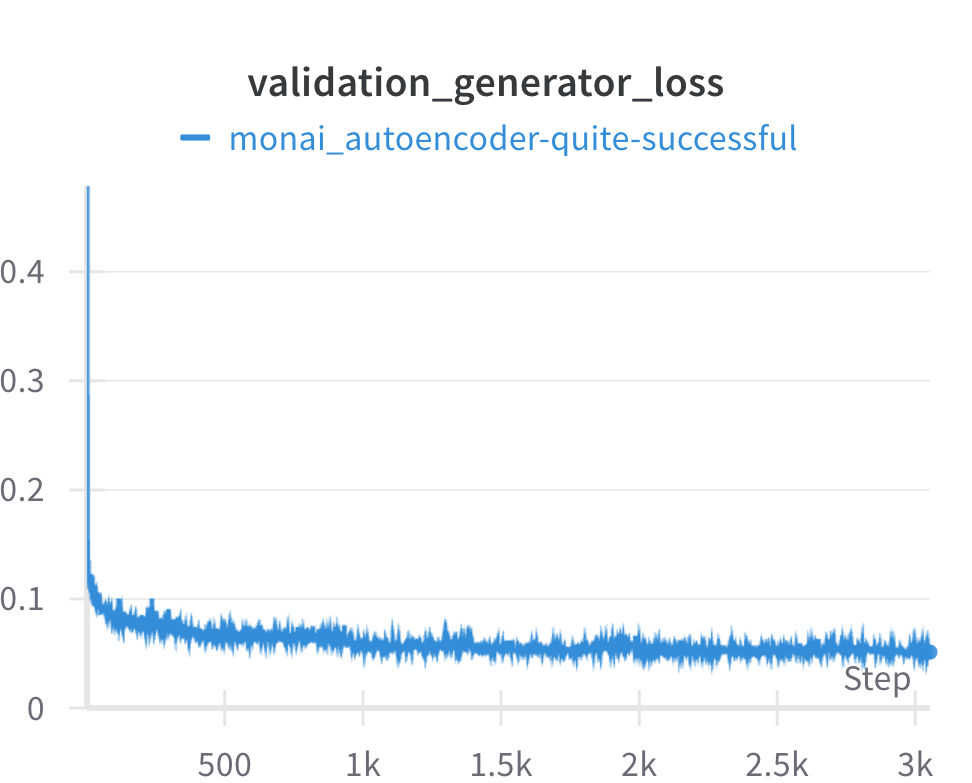
\includegraphics[width=\linewidth]{detailed_engineering/Monai Autoencoder/charts/val_generator_loss.png}
\caption{}
\endminipage
\end{figure}


\paragraph{Results}\mbox{}\\

\begin{figure}[H]
    \centering
    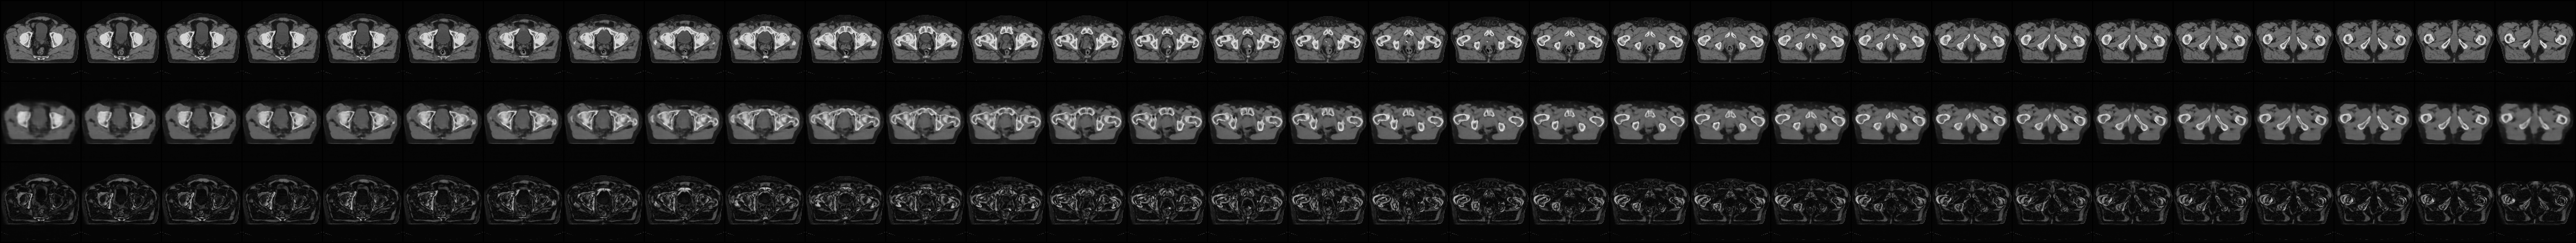
\includegraphics[width=\linewidth]{reports/monai_autoenc_comparison_full.png}
    \caption{Top - input, middle reconstruction, bottom difference.}
    \label{fig:enter-label}
\end{figure}

